\section{Performantie}
\label{sec:evaluatie-performantie}

%%%%%%%%%%%%

% Overzichtsgrafiek

% Volgens de POC is Lungo de winnaar, maar aangezien er niet alles is geïmplementeerd zou je kunnen denken dat daarom is, maar het duidelijkst is bij de loginschermen, alle 3 zijn quasi hetzelfde, behalve Lungo is een halvering van de tijd (dit omdat de geoptimaliseerde JS bibliotheek)
% De tweede plaats gaat naar jQM, volgend door Kendo en als laatste ST

% jQM, Kendo, Lungo gebruiken enkel HTML5 application cache, maar ST gebruikt daarna nog iets speciaals, zie sectie ST 
% Hierdoor wordt de grote laadtijd verklaard bij geachte versie van ST
% jQM, Kendo, Lungo zijn gelijkaardig doordat deze gebruikt worden gebouwd en uitgerold met Yeoman 
%%%% De cache factor van ST is constant (gemiddeld 1,8)
%%%% De andere raamwerken hebben een beduidend grotere cache factor 

% Algemeen de snelheden gecached versus niet gedaagde
% De eerste keer laden van webappplicaties duurt gemiddeld 3,3s (niet voor ST)
% De gecachte versie openen duurt gemiddeld 400ms (niet voor ST), wat een aanvaardbare tijd is volgens http://www.nngroup.com/articles/response-times-3-important-limits/

% TODO Tim: tabel maken voor de dingen hieronder
% deze dingen uitdiepen hieronder
% page speed
% LOC
% download grootte (POC/login, 1 getal per framework, gemiddelde per device)
% subjectieve experience lijsten
% ST scoort het beste volgens google page speed, maar dat heeft dus te maken met die microlader, daarna volgt lungo, Kendo en jQM die de regels minder strikt, maar uiteindelijk toch sneller presteren

% jQM login<->POC: geen, de beste factor
% ST: immens verschil
% Lungo: zelfde factor als ST
% Kendo de tweede beste factor

% ST was de beste experience, op zowel oude als nieuwe toestellen
% dan volgt jquery mobile, dan lungo en dan kendo
% kendo crashes 
% link naar nelson http://www.nngroup.com/articles/why-you-only-need-to-test-with-5-users/

\begin{figure}
  \centering
  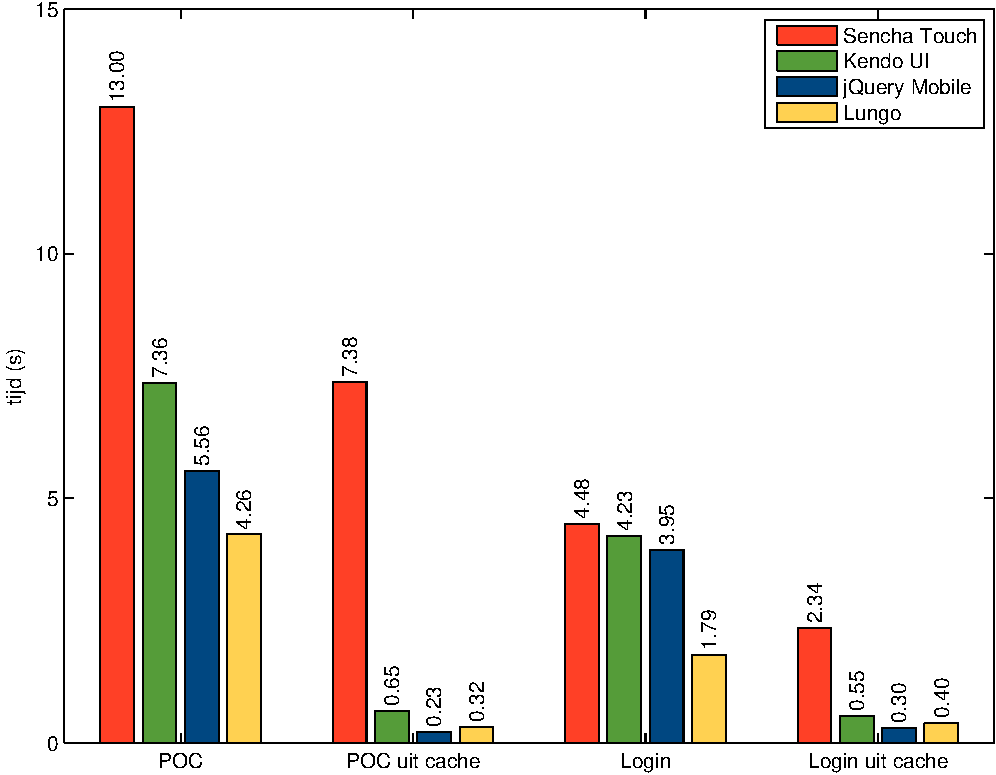
\includegraphics[width=0.8\textwidth]{figuren/performance.pdf}
  \caption{Downloadtijden voor POC,  POC uit cache,  Login en Login uit cache voor elk raamwerk.}
  \label{fig:performantie}
\end{figure}


\subsection{\st}
% individuele grafiek
% http://www.sencha.com/blog/behind-sencha-command-and-the-build-process

\begin{figure}
  \centering
  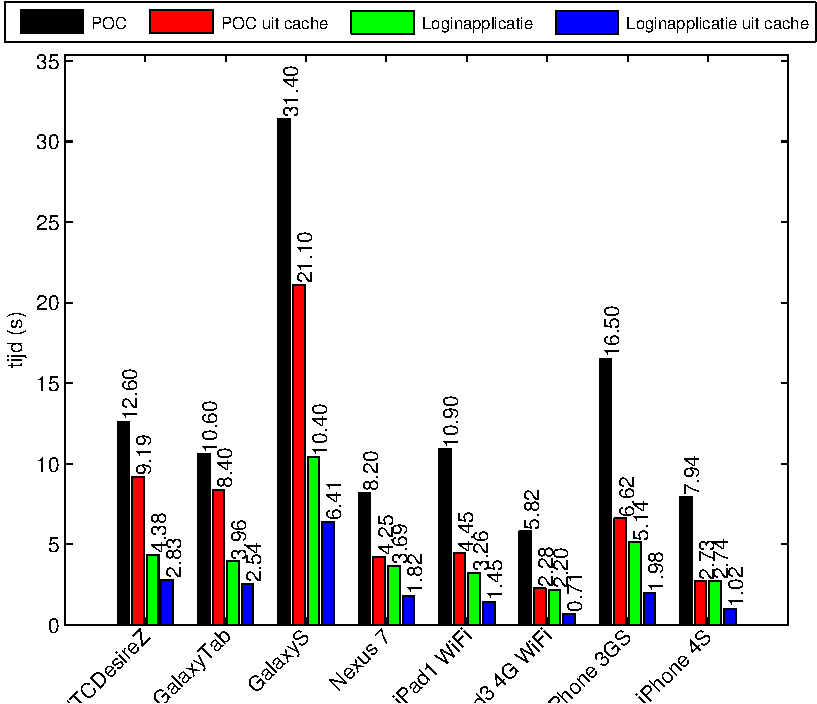
\includegraphics[width=0.5\textwidth]{figuren/performance-st.pdf}
  \caption{Downloadtijden van \st{} voor POC,  POC uit cache,  Login en Login uit cache voor elk device.}
  \label{fig:performantie-st}
\end{figure}

\subsection{\kendo}

\begin{figure}
  \centering
  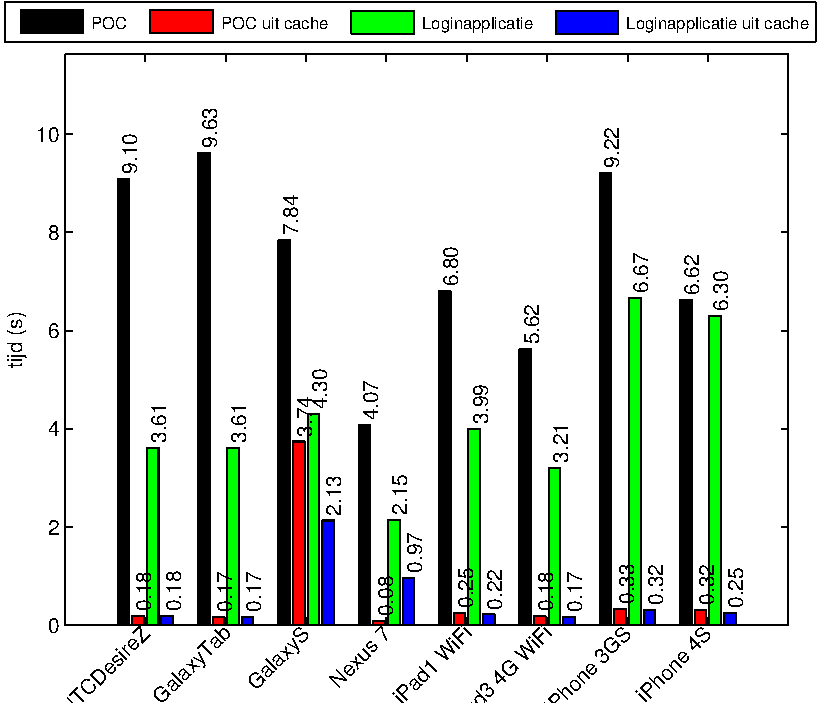
\includegraphics[width=0.5\textwidth]{figuren/performance-kendo.pdf}
  \caption{Downloadtijden van \kendo{} voor POC,  POC uit cache,  Login en Login uit cache voor elk device.}
  \label{fig:performantie-kendo}
\end{figure}

\subsection{\jqm}

\begin{figure}
  \centering
  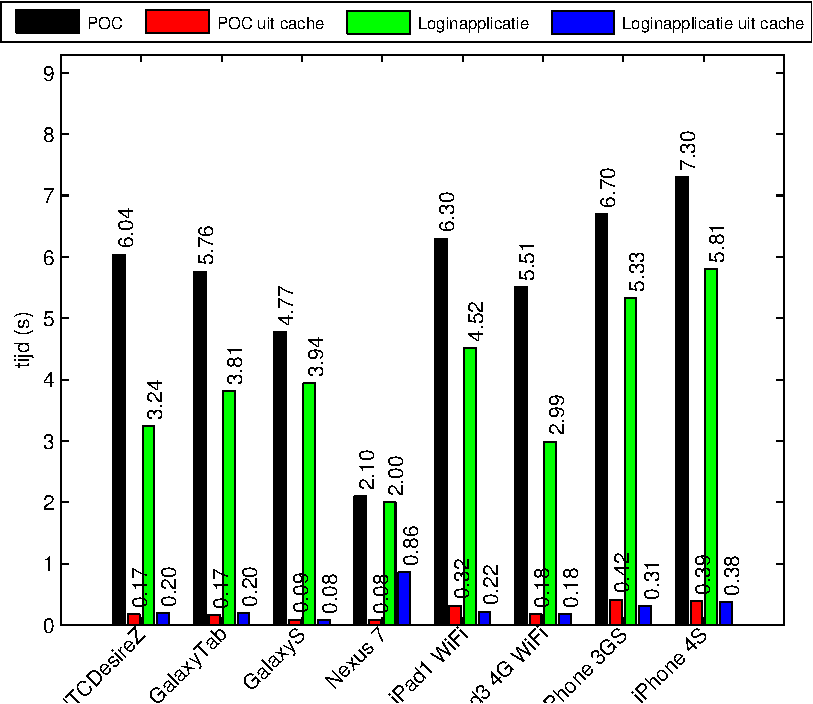
\includegraphics[width=0.5\textwidth]{figuren/performance-jquery.pdf}
  \caption{Downloadtijden van \jqm{} voor POC,  POC uit cache,  Login en Login uit cache voor elk device.}
  \label{fig:performantie-jqm}
\end{figure}

\subsection{\lungo}

\begin{figure}
  \centering
  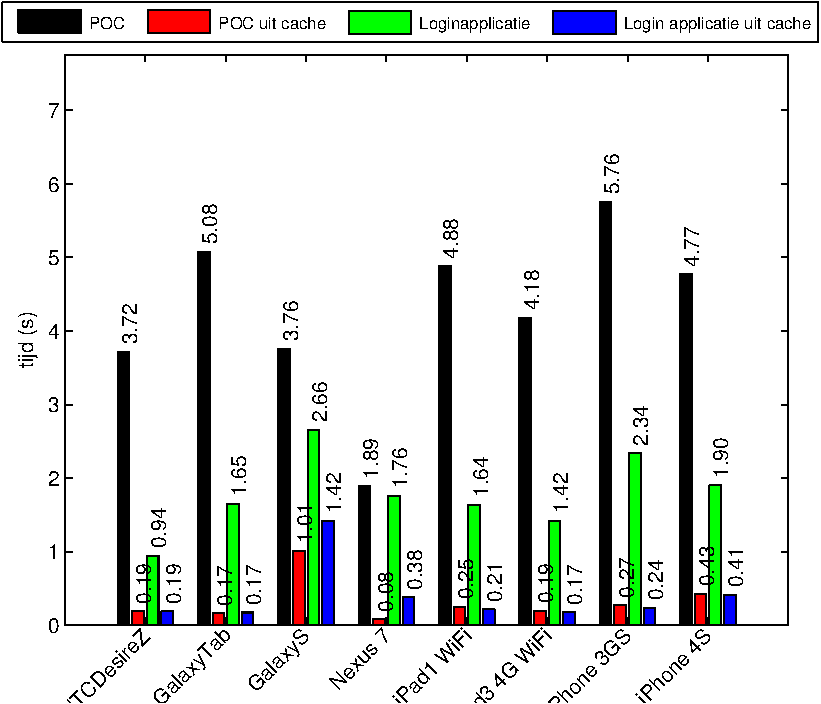
\includegraphics[width=0.5\textwidth]{figuren/performance-lungo.pdf}
  \caption{Downloadtijden van \lungo{} voor POC,  POC uit cache,  Login en Login uit cache voor elk device.}
  \label{fig:performantie-lungo}
\end{figure}
